\documentclass[10pt]{beamer}
\usepackage[english]{babel}
\setbeamertemplate{theorems}[numbered]
\setbeamertemplate{caption}[numbered]
\usefonttheme[onlymath]{serif}
\usetheme{Dallas}
\mode<presentation>
\setlength{\textwidth}{4.25in}
\parindent=0pt
\setlength{\parskip}{8pt}
\renewcommand{\baselinestretch}{1.0}

% Import graphics packages, set the graphics path
\usepackage{graphicx}
\graphicspath{{images/}}
\usepackage{subfig}
\usepackage{wrapfig}
\usepackage{multimedia}

\usepackage{changepage}

% Get rid of the navigation buttons
\setbeamertemplate{navigation symbols}{}

% % Add extra space under footnotes to make room for navigation buttons
% \addtobeamertemplate{footnote}{}{\vspace{2ex}}

% Import math packages
\usepackage{amssymb}
\usepackage{amsmath}
\usepackage{mathrsfs} % to use mathscr
\usepackage{dsfont}
\usepackage{physics}

% \usepackage[algo2e,ruled,vlined]{algorithm2e}
% \usepackage[]{algorithm2e}
\usepackage[ruled, vlined, linesnumbered, noend]{algorithm2e}
\usepackage{algorithmic}
\renewcommand{\algorithmicrequire}{\textbf{Input:}}
\renewcommand{\algorithmicensure}{\textbf{Output:}}
\usepackage{mathtools}

% Import packages for square, diamong, .. cirlces
\usepackage{fdsymbol}

% Define theorem-like environments


\SetKw{Return}{Return}
\SetKw{Find}{Find}
\SetKw{Define}{Define}

% Place the UTD logo in the frame titles
\usepackage{textpos}
\addtobeamertemplate{frametitle}{}{%
\begin{textblock*}{30mm}(.90\textwidth,-0.78cm)
% \includegraphics[height=0.7cm]{UT_Dallas_White.eps}
\end{textblock*}}
\addtobeamertemplate{frametitle}{}{%
\begin{textblock*}{30mm}(.73\textwidth,-0.75cm)
% \includegraphics[height=0.63cm]{conlab_logo_white_on_transparent.png}
% .73\textwidth: affects horizontal placement
% -0.75cm affects vertical placement
% [height=0.63cm] affects size of the image
\end{textblock*}}

% \begin{textblock*}{30mm}(.90\textwidth,-0.78cm)
% \includegraphics[height=0.7cm]{}
% \end{textblock*}

% Set the block styles
% Green
\setbeamercolor{block title}{use=structure,fg=white,bg=structure.fg}
\setbeamercolor{block body}{use=structure,fg=black,bg=structure.fg!3}
% Orange
% \setbeamercolor{block title}{use=structure,fg=white,bg=structure.bg}
% \setbeamercolor{block body}{use=structure,fg=black,bg=structure.bg!3}

% Navigation Stuff
\addtobeamertemplate{navigation symbols}{}{%
	\usebeamerfont{footline}%
	\usebeamercolor[fg]{footline}%
	\hspace{1em}%
	\insertframenumber/\inserttotalframenumber
}


% Set the itemize-like environment styles
\setbeamercolor{item}{fg=structure.fg,bg=structure.bg}
\setbeamertemplate{bibliography item}{\insertbiblabel}
\setbeamertemplate{itemize items}[square]
\setbeamertemplate{enumerate items}[square]

% Change the itemize-like environment spacings
\makeatletter
\def\@listI{\leftmargin\leftmargini
            \parsep 1pt
            \topsep 1pt
            \itemsep 1pt
            \parskip 2pt}
\makeatother


\AtBeginSection[]
{
	\begin{frame}
		\frametitle{Table of Contents}
		\tableofcontents[currentsection]
	\end{frame}
}

\AtBeginSubsection[]
{
	\begin{frame}
		\frametitle{Table of Contents}
		\tableofcontents[currentsection,currentsubsection]
	\end{frame}
}




% Import definitions of command character sequences
%% Command definitions
% \def\i {\iota}
% mathbb
\def\bbb{\mathbb B}
\def\bbn{\mathbb N}
\def\bbz{\mathbb Z}
\def\bbq{\mathbb Q}
\def\bbr{\mathbb R}
\def\bbc{\mathbb C}
\def\bbs{\mathbb S}
\def\bbp{\mathbb P}
\def\bbe{\mathbb E}
%  mathbf
\def\bfx{\mathbf X}
\def\bfr{\mathbf R}
\def\bfs{\mathbf S}
% mathcal
\def\calx{\mathcal X}
\def\calu{\mathcal U}
\def\calr{\mathcal R}
\def\calp{\mathcal P}
\def\caln{\mathcal N}
\def\calf{\mathcal F}
\def\cali{\mathcal I}
\def\cald{\mathcal D}
\def\calo{\mathcal O}
\def\calc{\mathcal C}
\def\calt{\mathcal T}
\def\cals{\mathcal S}
% mathscr
\def\scrr{\mathscr R}
\def\scrp{\mathscr P}
\def\scrx{\mathscr X}
\def\scrt{\mathscr T}



%======== Abbreviations ==========================
\newcommand{\Max}{\max\limits_}
\newcommand{\Min}{\min\limits_}
\newcommand{\Sup}{\sup\limits_}
\newcommand{\Inf}{\inf\limits_}

\newcommand{\PP}{\mathbb{P}}
\newcommand{\EE}{\mathbb{E}}
\newcommand{\RR}{\mathbb{R}}
\newcommand{\XX}{\mathbb{X}}
\newcommand{\CC}{\mathbb{C}}
\newcommand{\BB}{\mathbb{B}}
\newcommand{\YY}{\mathbb{Y}}
\newcommand{\UU}{\mathbb{U}}
\newcommand{\NN}{\mathbb{N}}

\newcommand{\Ru}{\overline {\R}}
\newcommand{\Rl}{\underline {\R}}
\newcommand{\borel}{\mathfrak{B}}

\newcommand{\lra}{\longrightarrow}
\newcommand{\Lra}{\Longrightarrow}
\newcommand{\Lla}{\Longleftarrow}
\newcommand{\Llra}{\Longleftrightarrow}
\newcommand{\ra}{\rightarrow}
\newcommand{\da}{\downarrow}
\newcommand{\ua}{\uparrow}
\newcommand{\rra}{\rightrightarrows}
\newcommand{\ora}{\protect\overrightarrow}


\newcommand{\ind}{\mathds{1}}
\newcommand{\Let}{: =}
\newcommand{\teL}{= :}
\newcommand{\diff}{\mathrm{d}}
\newcommand{\mn}{\wedge}
\newcommand{\mx}{\vee}
\newcommand{\ol}[1]{\overline{#1}}
\newcommand{\wt}{\widetilde}
\newcommand{\wb}{\widebar}
\newcommand{\shift}{\vartheta}
\newcommand{\com}{\circ}
\newcommand{\tp}{\intercal}
\newcommand{\opt}{\star}
\newcommand{\ball}[2]{\mathsf{B}_{#2}(#1)}		%{\mathbb{B}\left(#1;#2\right)}
\newcommand{\ballC}{\overline{\mathsf{B}}}
\newcommand{\ballO}{\mathsf{B}}
\newcommand{\bigO}{\mathcal{O}}

\newcommand{\eqsmall}[1]{{\small $#1$}}
\newcommand{\goodgap}{\hspace{\subfigtopskip}}

\newcommand{\eps}{\varepsilon}
\DeclareMathOperator{\esup}{esssup}
\newcommand{\conv}{\mathsf{conv}}


\DeclareMathOperator{\vect}{vec}
% \DeclareMathOperator{\Tr}{Tr}

\DeclareMathOperator*{\argmax}{arg\,max}
\DeclareMathOperator*{\argmin}{arg\,min}

\newcommand{\RRT}{RRT}
\newcommand{\RRTs}{RRT*}
\newcommand{\ransrrt}{RANS-RRT*}


% Colors
\newcommand{\bbar}[1]{\bar{\bar{#1}}}
\renewcommand{\r}[1]{{\color{red}{#1}}}
\renewcommand{\b}[1]{{\color{blue}{#1}}}
\newcommand{\p}[1]{{\color{purple}{#1}}}
\newcommand{\g}[1]{{\color{OliveGreen}{#1}}}


%  Math 
\newcommand{\trnsp}[1]{{#1}^T}
\newcommand{\inv}[1]{{#1}^{-1}}
\newcommand{\invpar}[1]{\left ( {#1} \right) ^{-1}}
\newcommand{\invbrack}[1]{\left [ {#1} \right ] ^{-1}}

\newcommand{\absval}[1]{\mid {#1} \mid}
\newcommand{\innerprod}[1]{\langle {#1} \rangle}
% \newcommand{\norm}[1]{\left\lVert {#1} \right\rVert}
\newcommand{\rlbrack}[1]{\left [ {#1} \right]}
\newcommand{\rlbrace}[1]{\left \{ {#1}  \right\}}
\newcommand{\rlpar}[1]{\left ( {#1} \right)}

\newcommand{\matg}{\succ}
\newcommand{\matl}{\prec}
\newcommand{\matgeq}{\succeq}
\newcommand{\matleq}{\preceq}

\newcommand{\mean}[1]{\overline{{#1}}}
\newcommand{\expect}[1]{\bbe \rlbrack{{#1}}}



% Temporal Logic Operators
% Until
\newcommand{\until}[2]{\mathscr{U}_{[{#1},{#2}]}} % until with closed interval [a,b]
\newcommand{\untilI}[1]{\mathscr{U}_{{#1}}} % until with interval I
% Eventually
\newcommand{\finally}[2]{\mathscr{F}_{[{#1},{#2}]}} % eventually operator as F (finally) with closed interval [a,b]
\newcommand{\finallyI}[1]{\mathscr{F}_{#1}} % eventually operator as F (finally) with interval I
\newcommand{\eventually}[2]{\diamondsuit_{[{#1},{#2}]}} % eventually operator as a rhombus with closed interval [a,b]
% Always
\newcommand{\globally}[2]{\mathscr{G}_{[{#1},{#2}]}} % always operator as G (globally) with closed interval [a,b]
\newcommand{\globallyI}[1]{\mathscr{G}_{#1}} % always operator as G (finally) with interval I
\newcommand{\always}[2]{\square_{[{#1},{#2}]}} % always operator as a square with closed interval [a,b]

% Gaussian Distribution
\newcommand{\gaussd}[2]{\mathcal{N}\rlpar{{#1}, {#2}}} 


%======== Theorems and Definitions ==========================
% \newtheorem{lemma}{Lemma}
% \newtheorem{remark}{Remark}
% \newtheorem{prop}{Proposition}
% \newtheorem{theorem}{Theorem}
% \newtheorem{corollary}{Corollary}
% \newtheorem{conjecture}{Conjecture}
% \newtheorem{assump}{Assumption}
% \theoremstyle{definition}
% \newtheorem{example}{Example}
% \newtheorem{problem}{Problem}
% \newtheorem{definition}{Definition}


\newtheorem{lemmaN}{Lemma}
\newtheorem{remark}{Remark}
\newtheorem{prop}{Proposition \propnumber}
\newtheorem{theoremN}{Theorem}
\newtheorem{corollaryN}{Corollary}
\newtheorem{conjecture}{Conjecture}
\newtheorem{assump}{Assumption}
\theoremstyle{definition}
\newtheorem{examp}{Example}
\newtheorem{problemN}{Problem}
\newtheorem{definitionN}{Definition}

\newcommand{\propnumber}{} % initialize
\newenvironment{propc}[1]
  {\renewcommand{\propnumber}{#1}%
   \begin{prop}}
  {\end{prop}}
\newtheorem{exercise}{Exercise}


\DeclareMathOperator{\reshape}{reshape}
\DeclareMathOperator{\gare}{gare}

% Double underscore without spaces i.e. for writing Python __init__, __main__, etc.
\newlength\dunder
\settowidth{\dunder}{\_}
\newcommand{\twound}{\rule{2\dunder}{0.4pt}}

% Bold rich color
% Green
\def\bgr{\em\bf\color{UTDseafoam!75!UTDgreen}} % light green
\def\bdgr{\em\bf\color{UTDseafoam!50!UTDgreen}} % dark green
% Orange
\def\bor{\em\bf\color{UTDorange!50!orange}} % orange
% Math version of bor and bdgr
\def\mor{\color{UTDorange!50!UTDorange}} % orange
\def\mdgr{\color{UTDseafoam!50!UTDgreen}} % green
\def\mdsf{\color{UTDseafoam!50!UTDseafoam}} % seafoam






%Logo and Image Packages
\usepackage{graphicx}
\logo{
\includegraphics[width=1.5in]{Images/UT_Dallas_Logo}}

%Additional Packages
\usepackage{physics}
\usepackage{setspace}

%Presentation Info
\title[Network Analysis of FRC Matches]{Match Structures Changes as the FIRST Robotics Competition Program Evolved}
\subtitle{Network Analysis of FRC Matches}
\author{Jonas Wagner}
\institute[UTDallas]{Univeristy of Texas at Dallas}
\date[2021-05-07]{SYSM 6302 Final Project\\ 2021 May 7th}




% The whole document
\begin{document}
\begin{frame}
	\titlepage
\end{frame}

\section{Background on FRC Matches}
\begin{frame}{FIRST Robotics Competition}
	\begin{columns}
		\column{0.55\textwidth}
			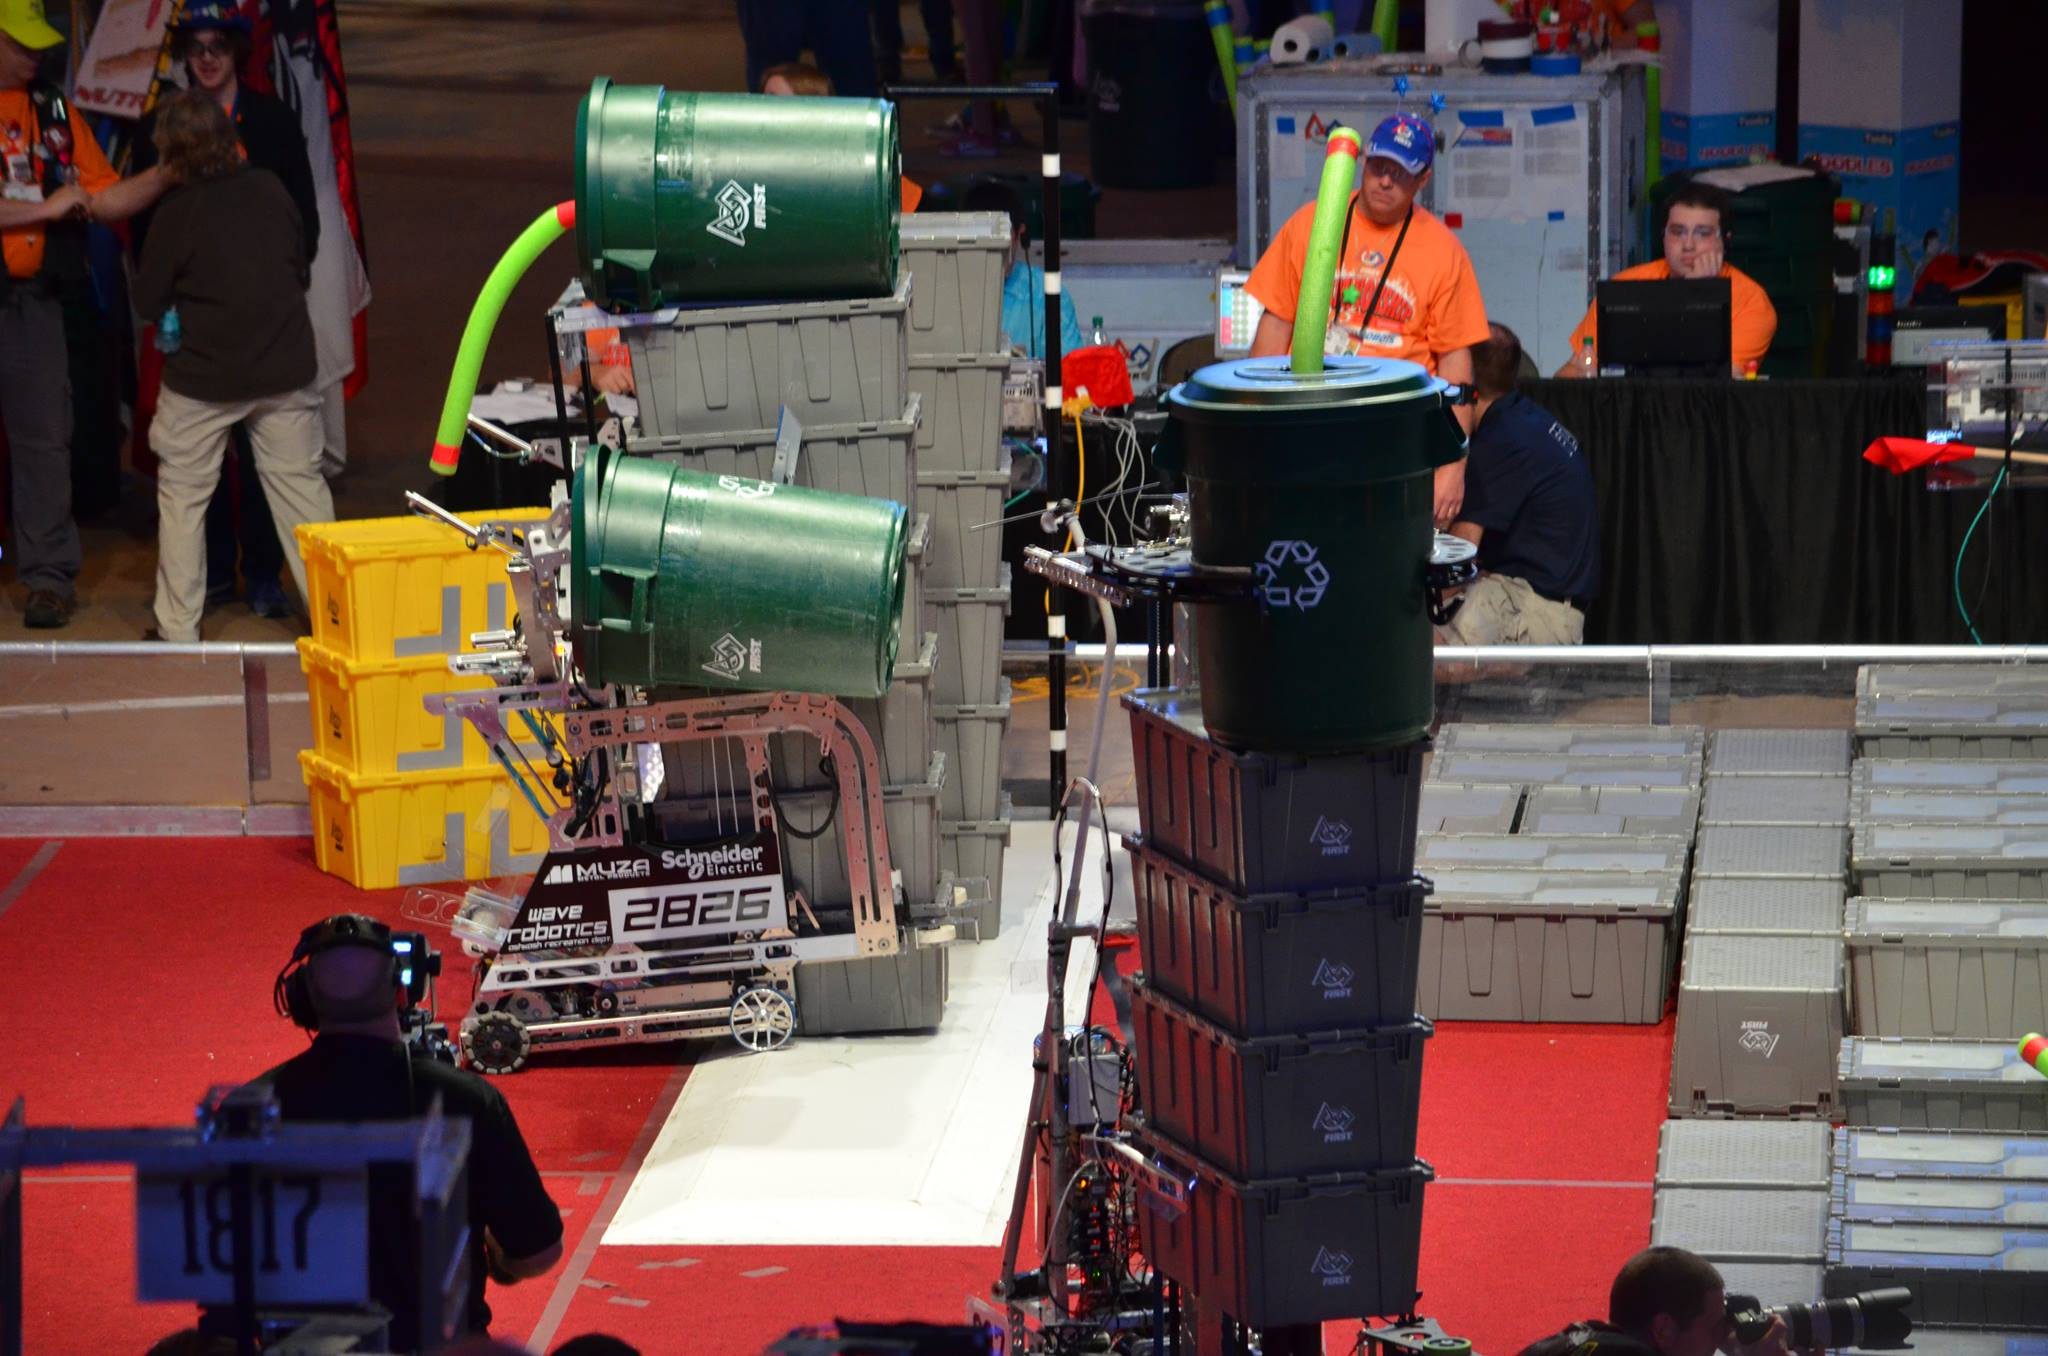
\includegraphics[width=\columnwidth]{Images/frc2826_2015}\\
			{\scriptsize FRC 2826 - Wave Robotics - Oshkosh, WI\\ World Championship Finalists 2015\\}
		\column{0.55\textwidth}
			
\includegraphics[width=0.4\columnwidth]{Images/frc_logo}
			{\centering
			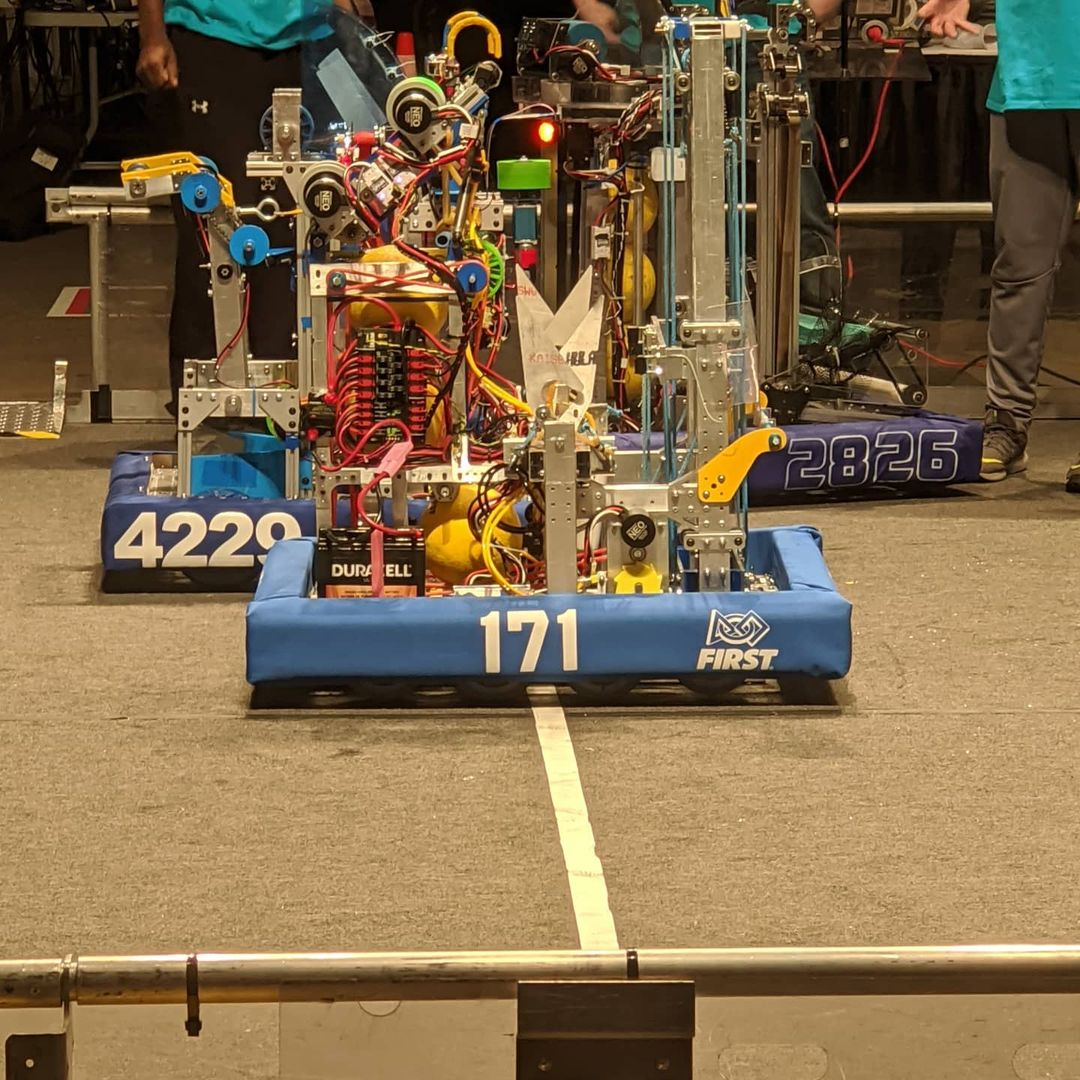
\includegraphics[width=0.8\columnwidth]{Images/frc171_2020}}\\
			{\scriptsize FRC 171 - The Cheese Curd Herd - Platteville, WI\\ Northern Lights Regional 2020 (Duluth, MI)\\}
			\vspace{0.2in}
	\end{columns}
\end{frame}

%\begin{frame}{Current Event Match Structure}
%	
%\end{frame}

%------------------------------------------------------------
\section{Data Collection and Network Construction}
%------------------------------------------------------------
\begin{frame}{The Blue Alliance}{www.thebluealliance.com   \cite{thebluealliance}}
	\begin{columns}
		\column{0.8\textwidth}
			The Blue Alliance is a very useful online database of past (and current) match data.\\
			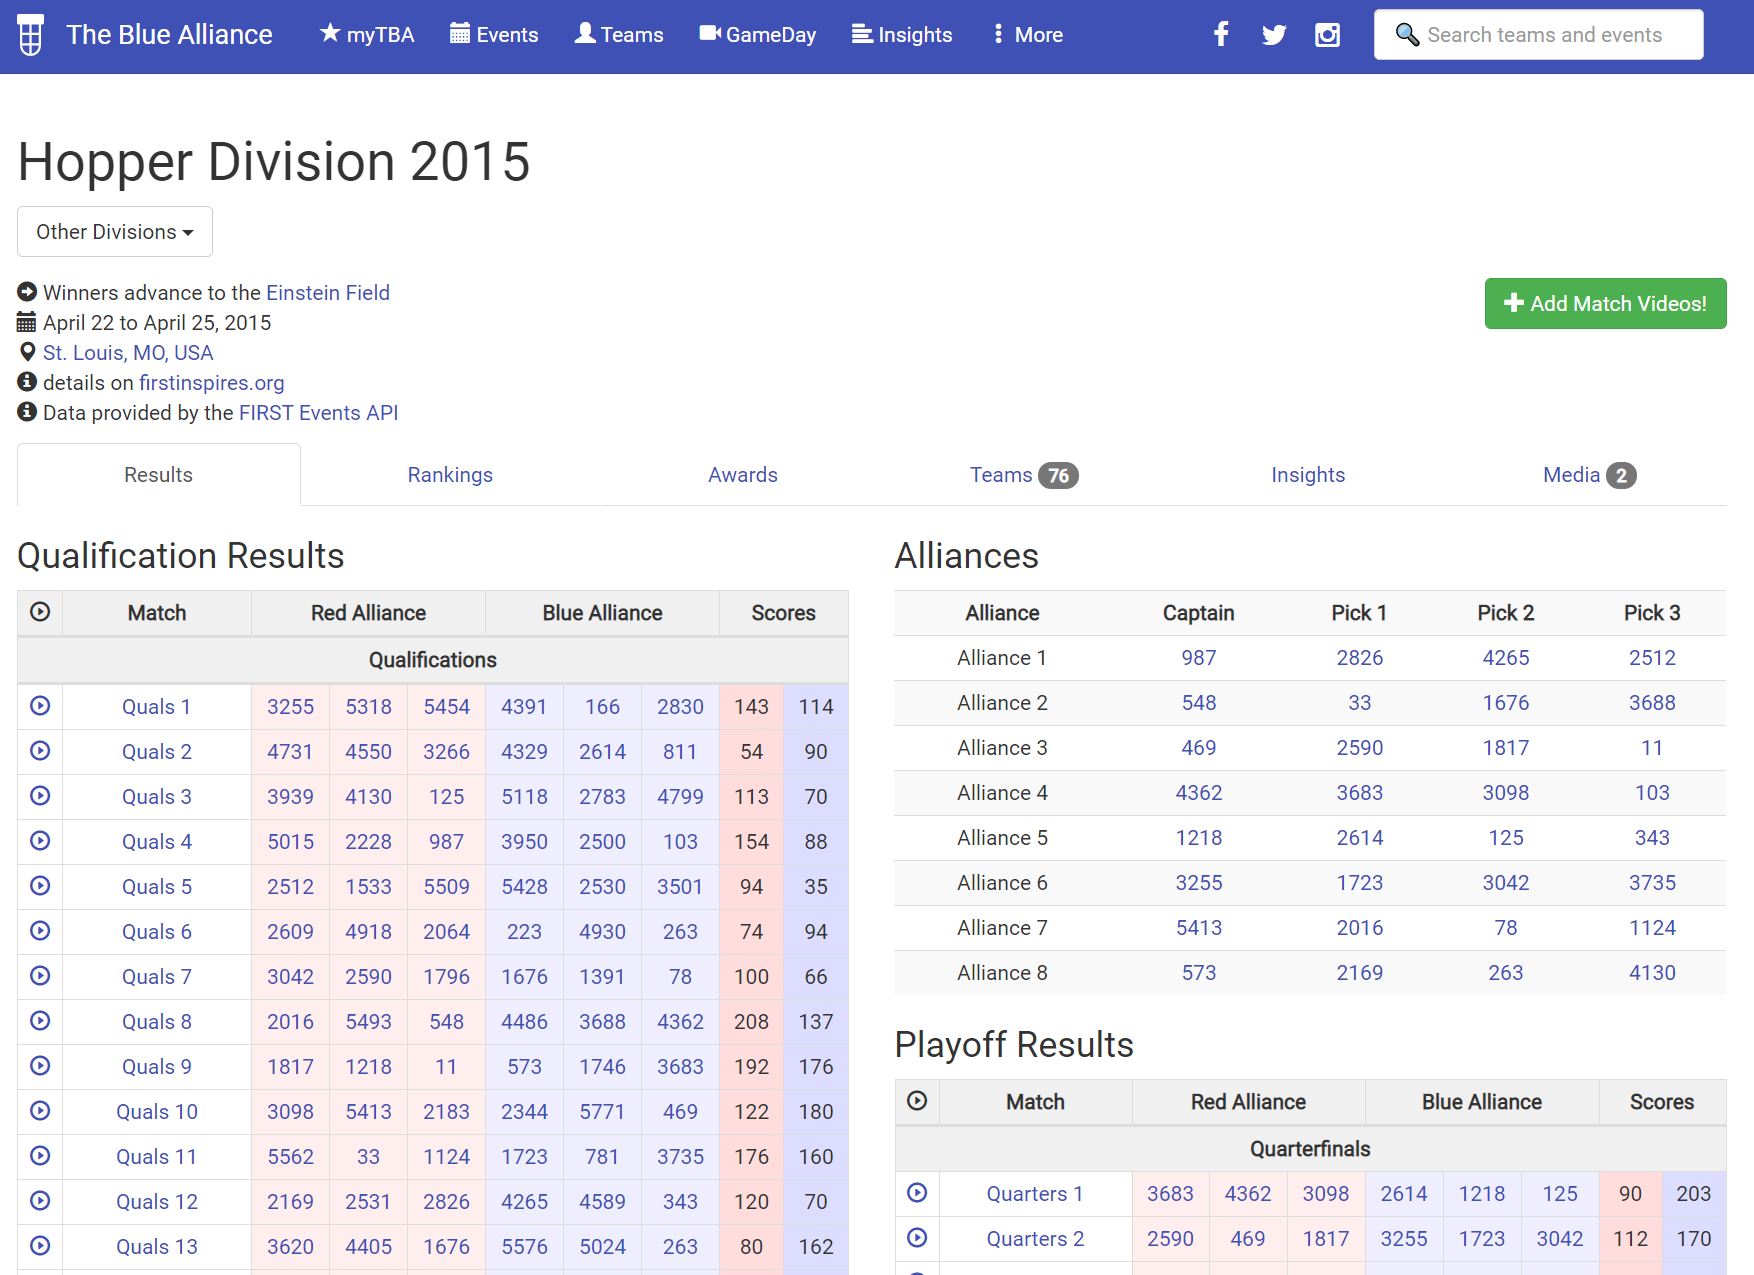
\includegraphics[height=0.5\textheight]{Images/tba_website}
		\column{0.2\textwidth}
			
\includegraphics[width=\columnwidth]{Images/tba_logo}
	\end{columns}
\end{frame}

%------------------------------------
\subsection{TBA\_Database\_Access.py}
%------------------------------------
\begin{frame}{Accessing The Blue Alliance Database}
	\begin{columns}
		\column{0.55\textwidth}
			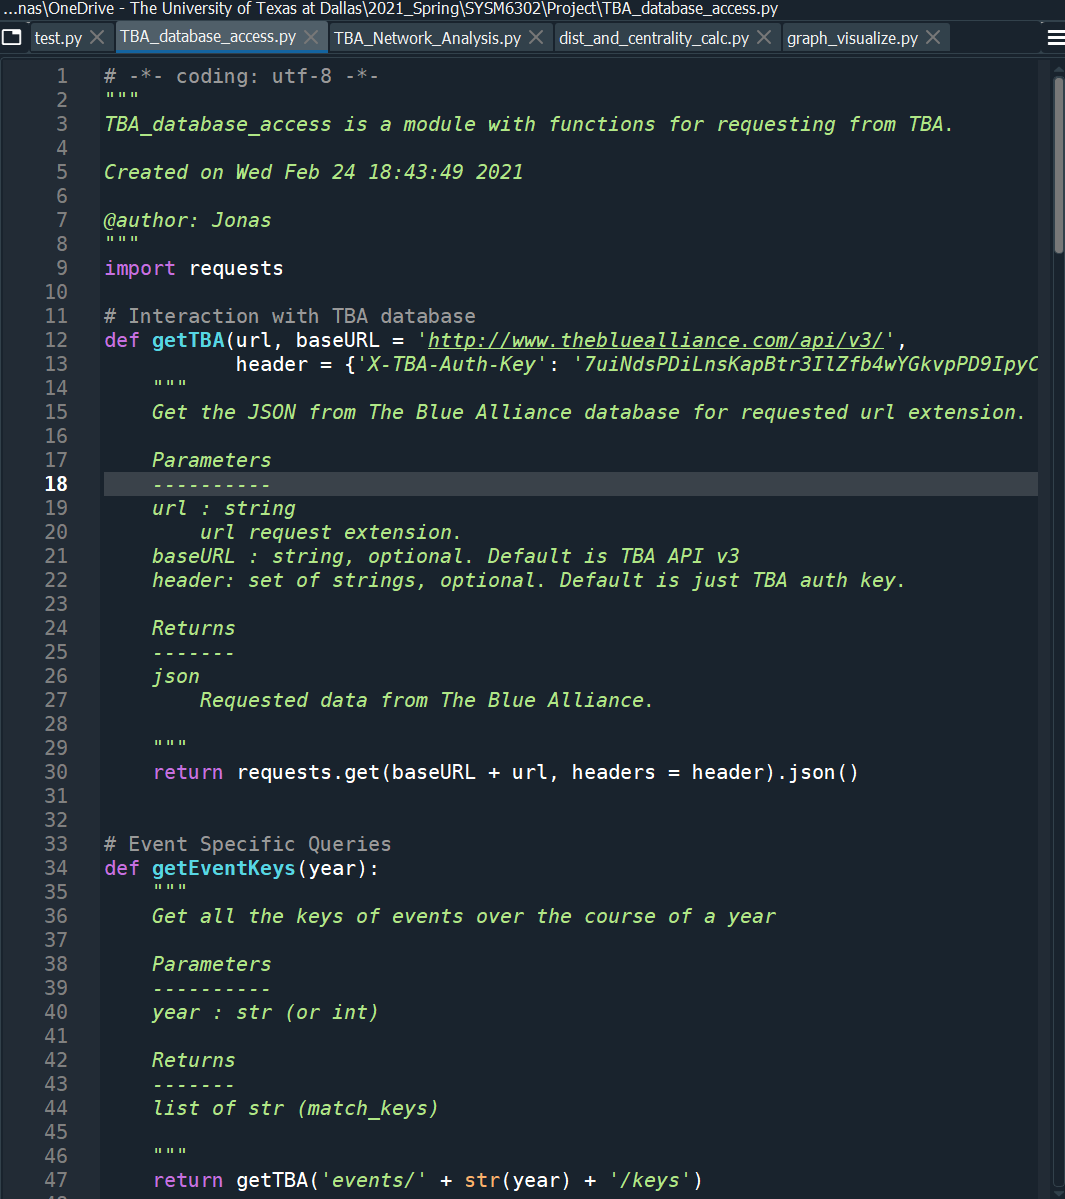
\includegraphics[width=\columnwidth]{Images/tba_database_access_screenshot1}
		\column{0.55\textwidth}
			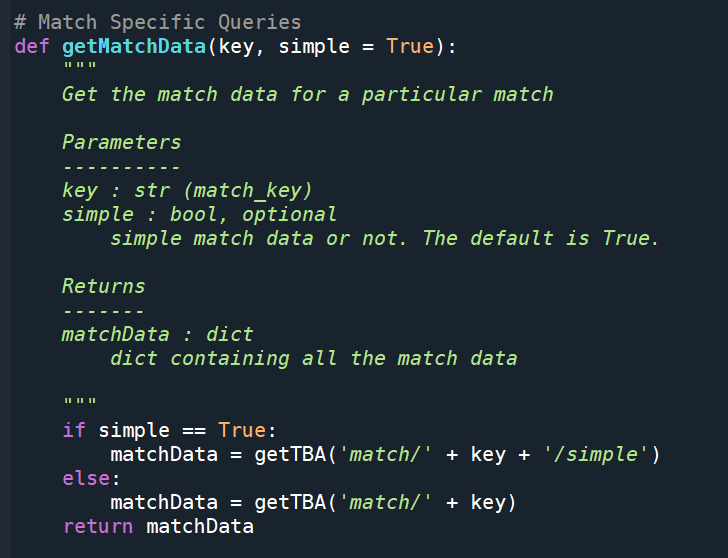
\includegraphics[width=\columnwidth]{Images/tba_database_access_screenshot2}\\
	%			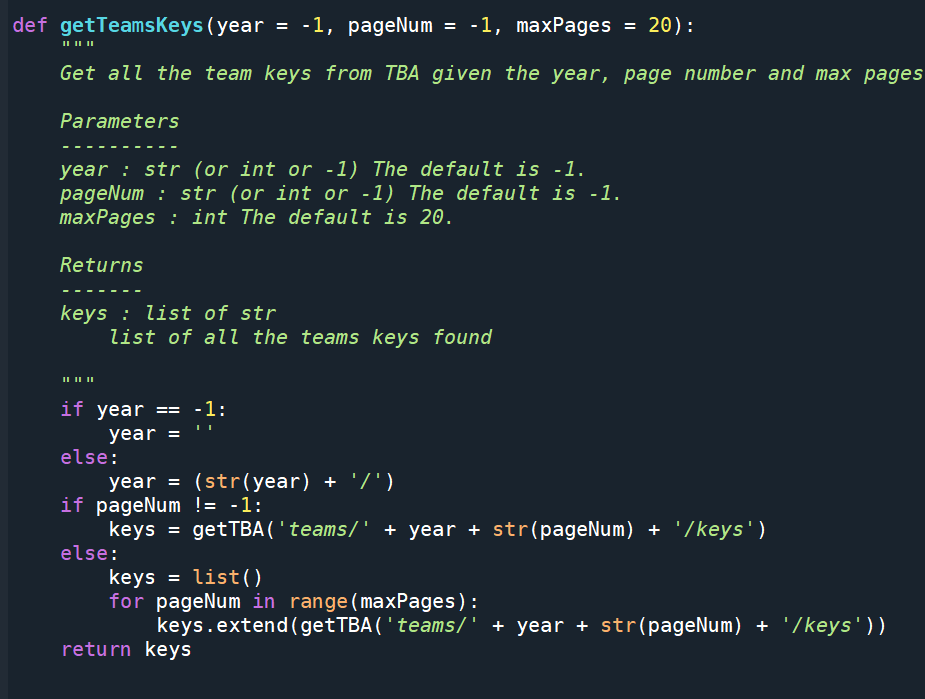
\includegraphics[width=\columnwidth]{Images/tba_database_access_screenshot3}
	\end{columns}
\end{frame}

%-------------------------------------
\subsection{TBA\_Network\_Analysis.py}
%--------------------------------------
\begin{frame}{Network Generation}
	\begin{columns}
		\column{0.55\textwidth}
			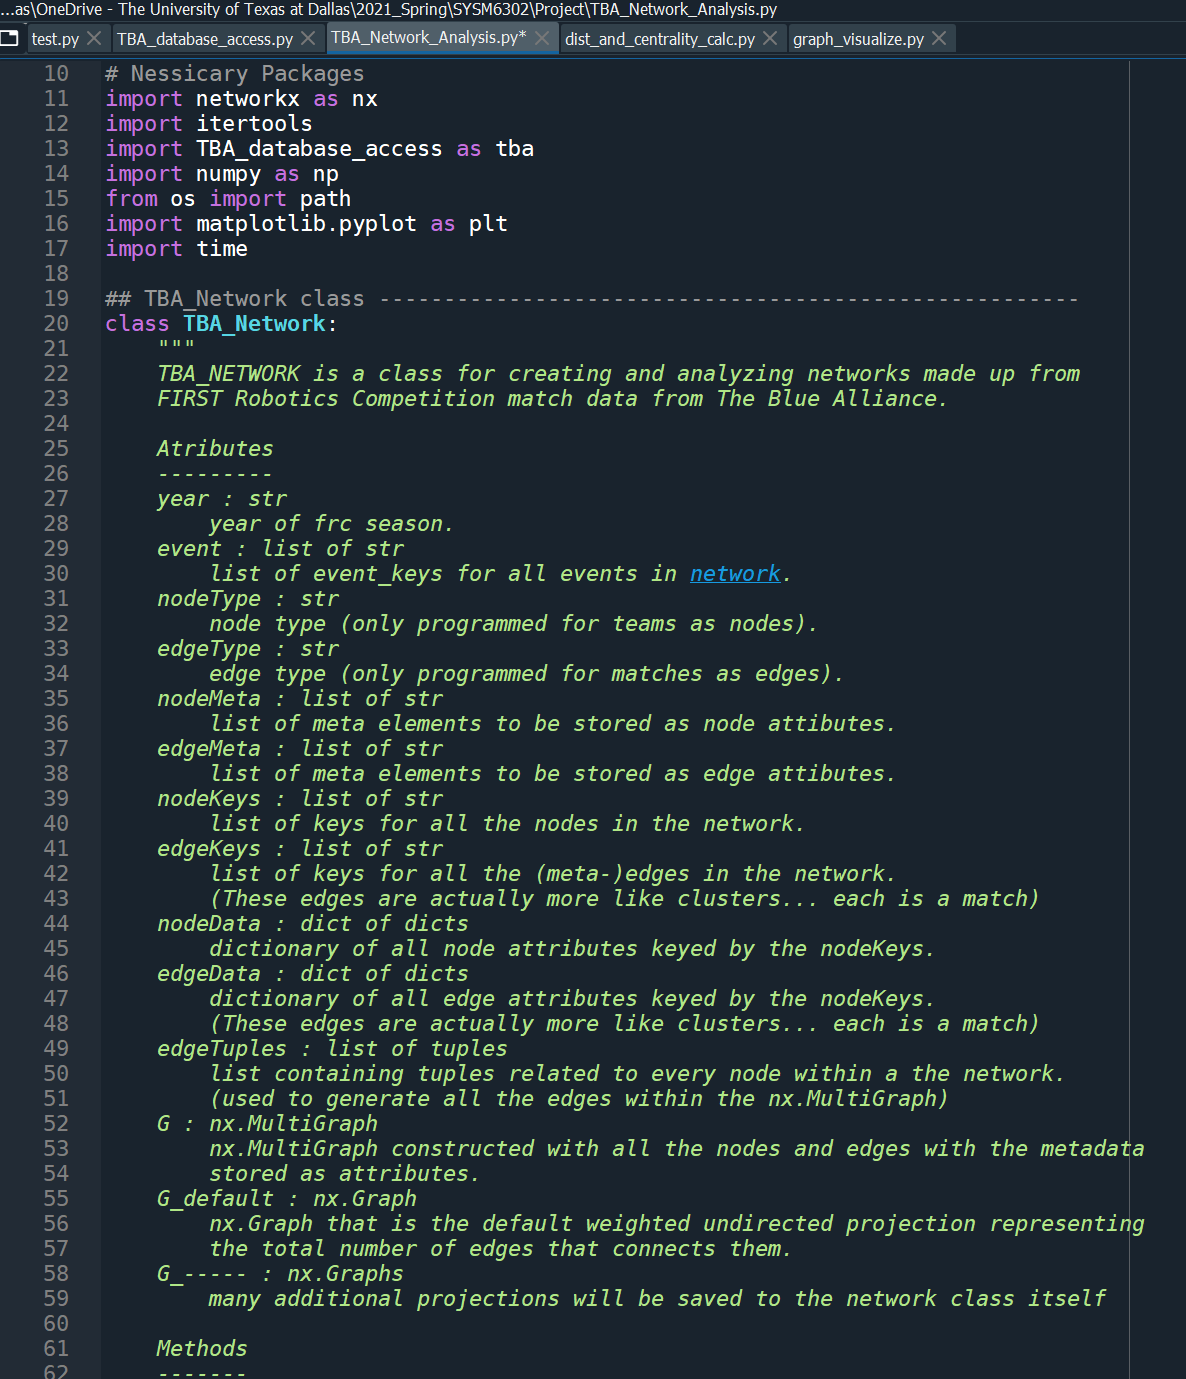
\includegraphics[width=\columnwidth]{Images/tba_network_analysis_screenshot1}
		\column{0.55\textwidth}
			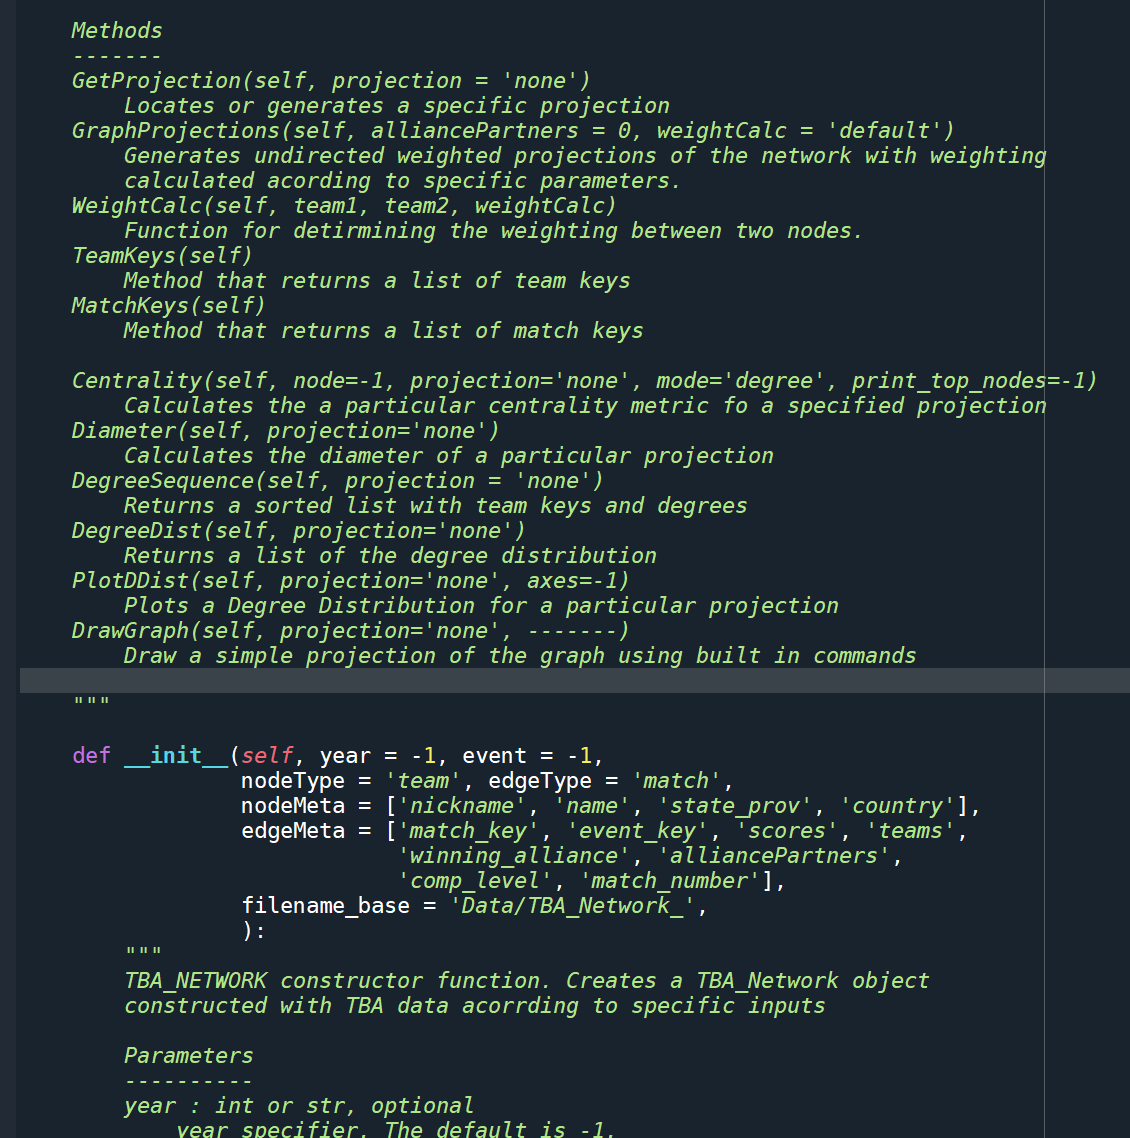
\includegraphics[width=\columnwidth]{Images/tba_network_analysis_screenshot2}
	\end{columns}
\end{frame}

%-------------------------------------
\subsection{Generated Network}
%--------------------------------------
\begin{frame}{Multi-Graph Produced}{2015 (my favorite season)}
	\begin{columns}
		\column{0.55\textwidth}
			
			
			
			\begin{itemize}
				\item Network: Entire 2015 Season
				\begin{itemize}
					\item TBA\_Network\_2015.gml
				\end{itemize} 
				\item Size: (45 MB)
				\begin{itemize}
					\item Nodes: 2,935 Teams
					\item Total Edges: 195,152
					\item Distinct Edges: 106,889
				\end{itemize}
				\item Components: 1
				\item Diameter: 4
			\end{itemize}
		\column{0.4\textwidth}
		\includegraphics[height=1\textheight]{../fig/NetworkPlot_2015}
	\end{columns}
\end{frame}

%\begin{frame}{Network Methods}
%	content...
%\end{frame}

%--------------------------------------------------------
\section{Analysis Results}
%------------------------------------------------------
\subsection{Basic Analysis on Event Projections}
%----------------------------------------
\begin{frame}{2015 Wisconsin Regional Analysis}{Milwaukee, WI}
	\begin{columns}
		\column{0.35 \textwidth}
		\includegraphics[height=0.85\textheight]{../fig/Centrality_Screenshot_2015wimi}
		\column{0.3 \textwidth}
		\includegraphics[height=0.85\textheight]{../fig/DegreeDist_2015wimi}
		\column{0.3 \textwidth}
		\includegraphics[height=0.85\textheight]{../fig/NetworkPlot_2015wimi}
	\end{columns}
\end{frame}
\begin{frame}{2015 Hopper Sub-Division Analysis}{FIRST Championships 2015: St. Louis, MO}
	\begin{columns}
		\column{0.35 \textwidth}
		\includegraphics[height=0.85\textheight]{../fig/Centrality_Screenshot_2015hop}
		\column{0.3 \textwidth}
		\includegraphics[height=0.85\textheight]{../fig/DegreeDist_2015hop}
		\column{0.3 \textwidth}
		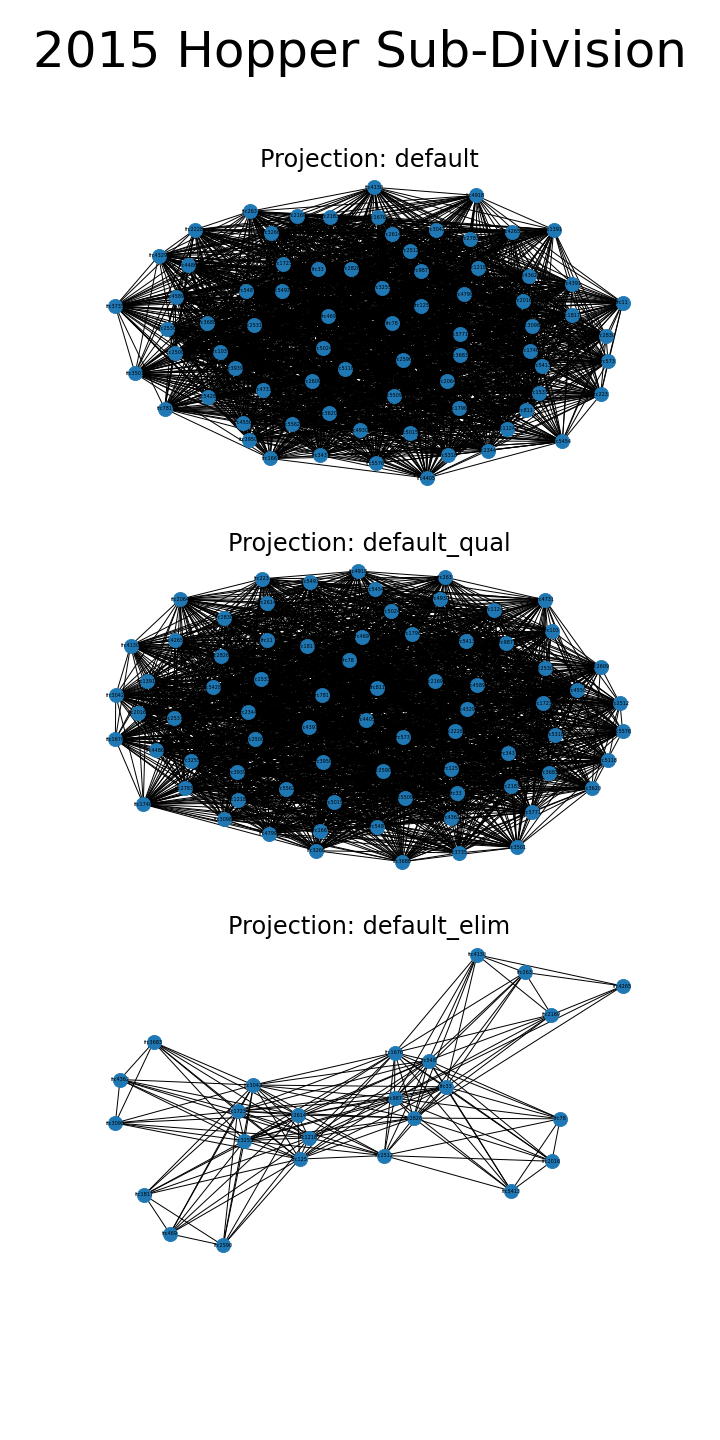
\includegraphics[height=0.85\textheight]{../fig/NetworkPlot_2015hop}
	\end{columns}
\end{frame}
\begin{frame}{2015 Einstein Analysis}{FIRST Championships 2015: St. Louis, MO}
	\begin{columns}
		\column{0.35 \textwidth}
		\includegraphics[height=0.85\textheight]{../fig/Centrality_Screenshot_2015cmp}
		\column{0.45 \textwidth}
		\includegraphics[width = \columnwidth]{../fig/DegreeDist_2015cmp}\\
		\includegraphics[width = \columnwidth]{../fig/NetworkPlot_2015cmp}
	\end{columns}
\end{frame}
%------------------------------------------------------
\subsection{Evolution of the Wisconsin Regional}
%----------------------------------------
\begin{frame}{2003 Midwest Regional Analysis}{Pre-WI Regional: In Evanston, IL}
	\begin{columns}
		\column{0.35 \textwidth}
		\includegraphics[height=0.85\textheight]{../fig/Centrality_Screenshot_2003il}
		\column{0.3 \textwidth}
		\includegraphics[height=0.85\textheight]{../fig/DegreeDist_2003il}
		\column{0.3 \textwidth}
		\includegraphics[height=0.85\textheight]{../fig/NetworkPlot_2003il}
	\end{columns}
\end{frame}
\begin{frame}{2008 Wisconsin Regional Analysis}{Milwaukee, WI}
	\begin{columns}
		\column{0.35 \textwidth}
		\includegraphics[height=0.85\textheight]{../fig/Centrality_Screenshot_2008wi}
		\column{0.3 \textwidth}
		\includegraphics[height=0.85\textheight]{../fig/DegreeDist_2008wi}
		\column{0.3 \textwidth}
		\includegraphics[height=0.85\textheight]{../fig/NetworkPlot_2008wi}
	\end{columns}
\end{frame}
\begin{frame}{2014 Wisconsin Regional Analysis}{Milwaukee, WI}
	\begin{columns}
		\column{0.35 \textwidth}
		\includegraphics[height=0.85\textheight]{../fig/Centrality_Screenshot_2014wimi}
		\column{0.3 \textwidth}
		\includegraphics[height=0.85\textheight]{../fig/DegreeDist_2014wimi}
		\column{0.3 \textwidth}
		\includegraphics[height=0.85\textheight]{../fig/NetworkPlot_2014wimi}
	\end{columns}
\end{frame}
\begin{frame}{2015 Wisconsin Regional Analysis}{Milwaukee, WI}
	\begin{columns}
		\column{0.35 \textwidth}
		\includegraphics[height=0.85\textheight]{../fig/Centrality_Screenshot_2015wimi}
		\column{0.3 \textwidth}
		\includegraphics[height=0.85\textheight]{../fig/DegreeDist_2015wimi}
		\column{0.3 \textwidth}
		\includegraphics[height=0.85\textheight]{../fig/NetworkPlot_2015wimi}
	\end{columns}
\end{frame}
\begin{frame}{2016 Wisconsin Regional Analysis}{Milwaukee, WI}
	\begin{columns}
		\column{0.35 \textwidth}
		\includegraphics[height=0.85\textheight]{../fig/Centrality_Screenshot_2016wimi}
		\column{0.3 \textwidth}
		\includegraphics[height=0.85\textheight]{../fig/DegreeDist_2016wimi}
		\column{0.3 \textwidth}
		\includegraphics[height=0.85\textheight]{../fig/NetworkPlot_2016wimi}
	\end{columns}
\end{frame}
\begin{frame}{2019 Seven-Rivers Regional Analysis}{La Crosse, WI}
	\begin{columns}
		\column{0.35 \textwidth}
		\includegraphics[height=0.85\textheight]{../fig/Centrality_Screenshot_2019wila}
		\column{0.3 \textwidth}
		\includegraphics[height=0.85\textheight]{../fig/DegreeDist_2019wila}
		\column{0.3 \textwidth}
		\includegraphics[height=0.85\textheight]{../fig/NetworkPlot_2019wila}
	\end{columns}
\end{frame}

%------------------------------------------------------------------------
\subsection{Evolution of Elimination Rounds}
%-----------------------------------------------------------------------
\begin{frame}{Einstein (Championship) Matches}
	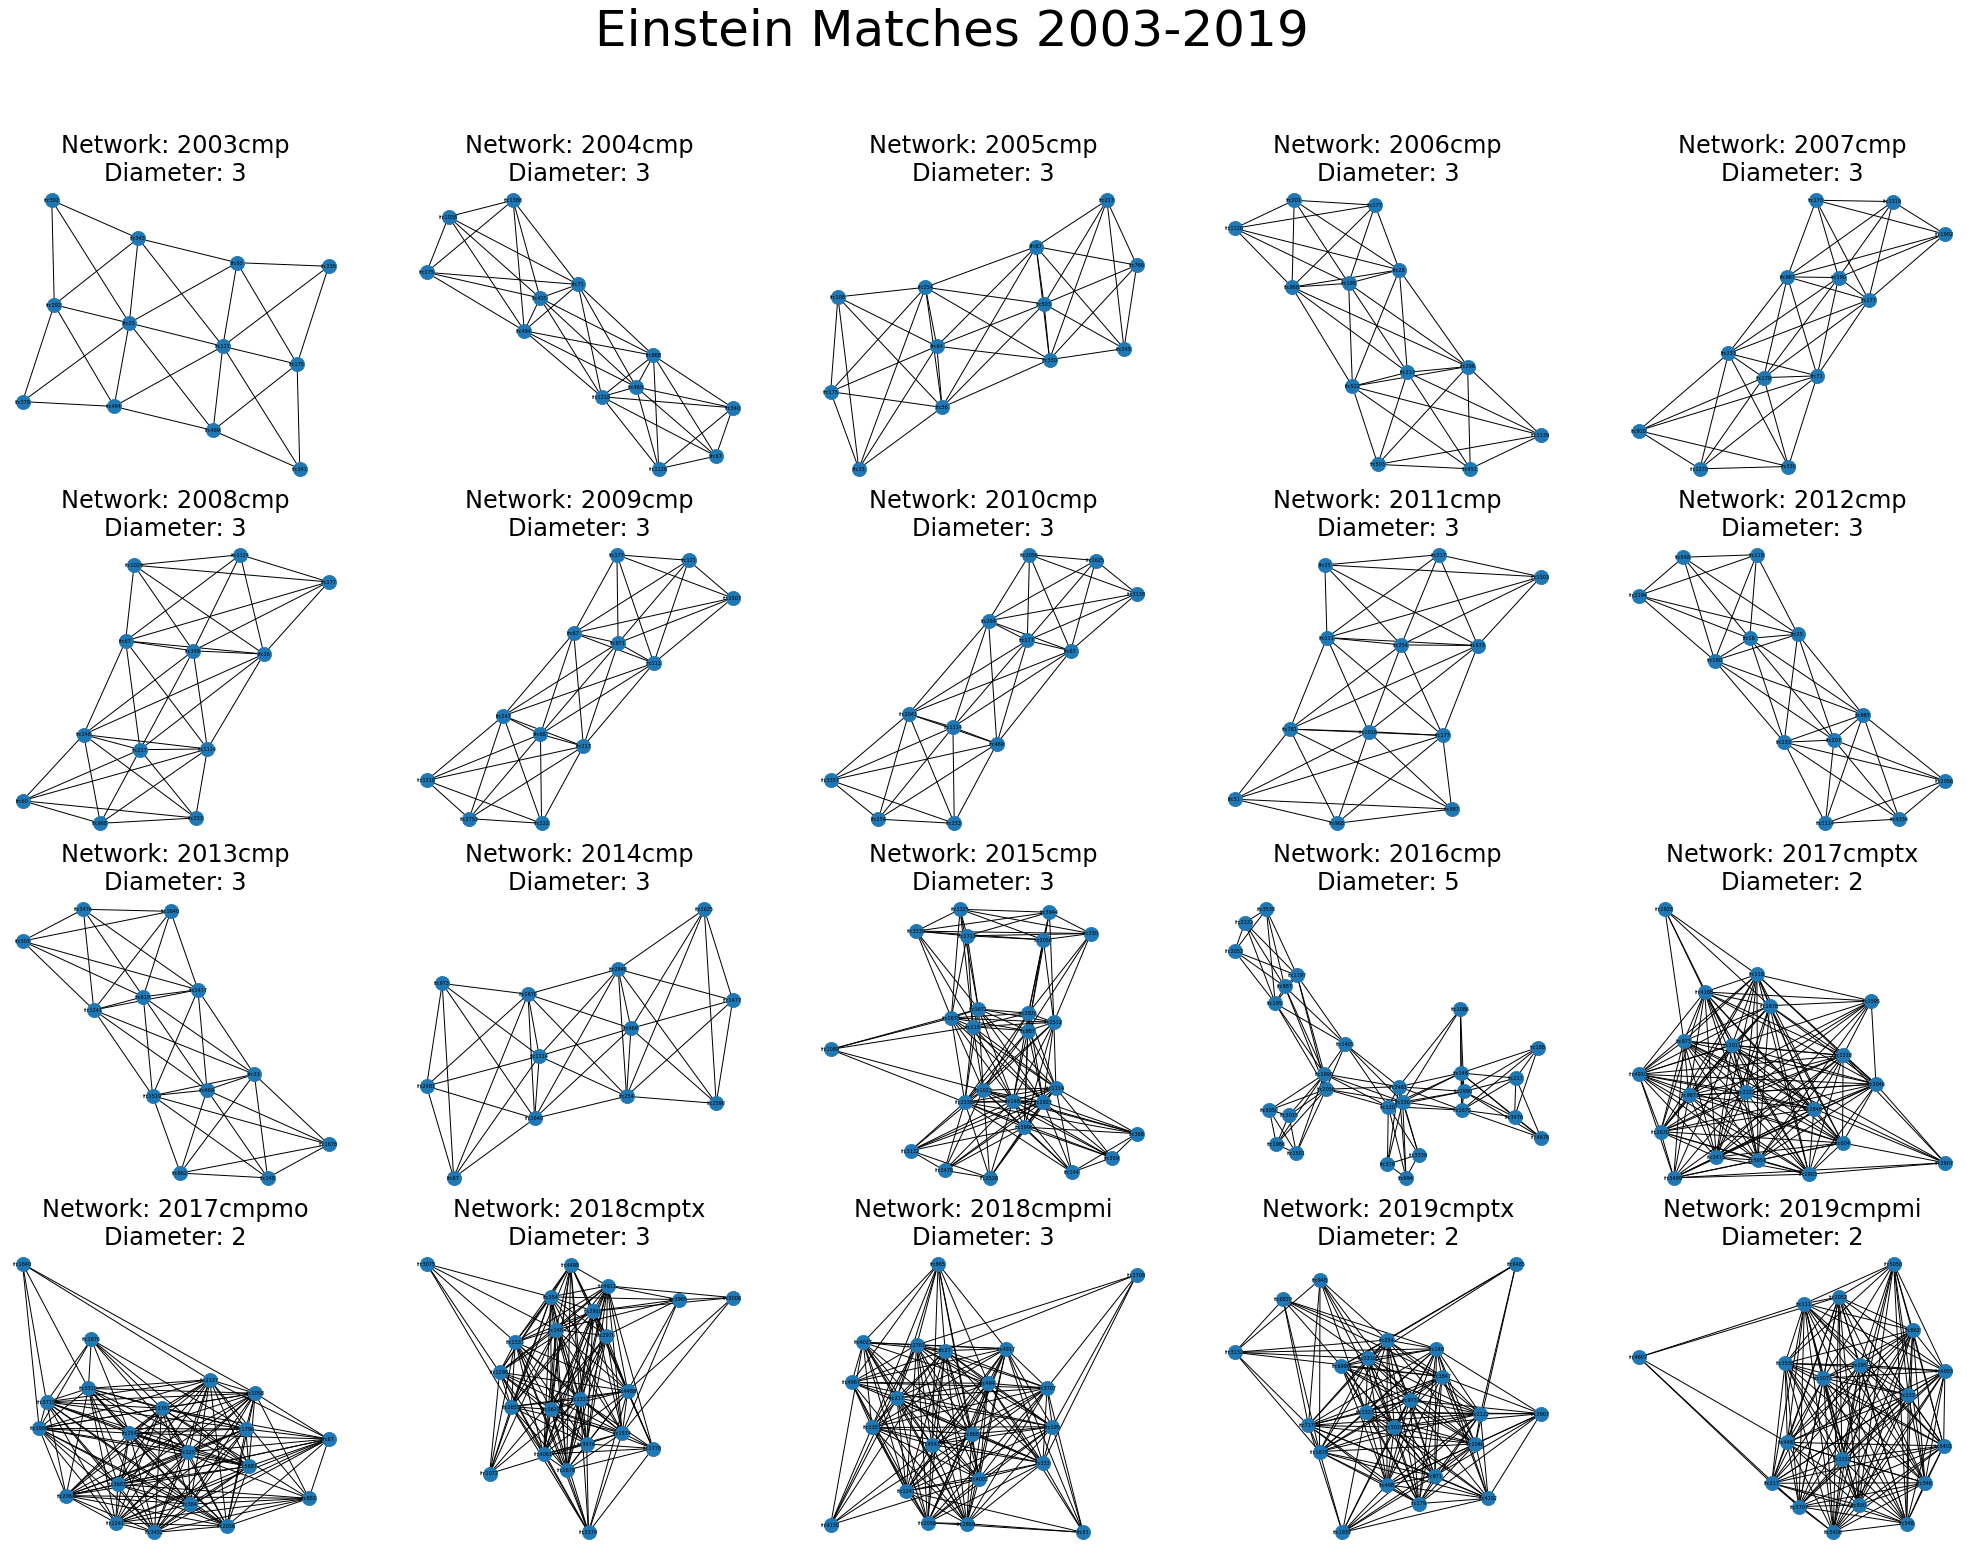
\includegraphics[height=0.85\textheight]{../fig/NetworkPlot_cmp_2003_2019}
\end{frame}
\begin{frame}{Einstein (Championship) Matches}
	\centering
	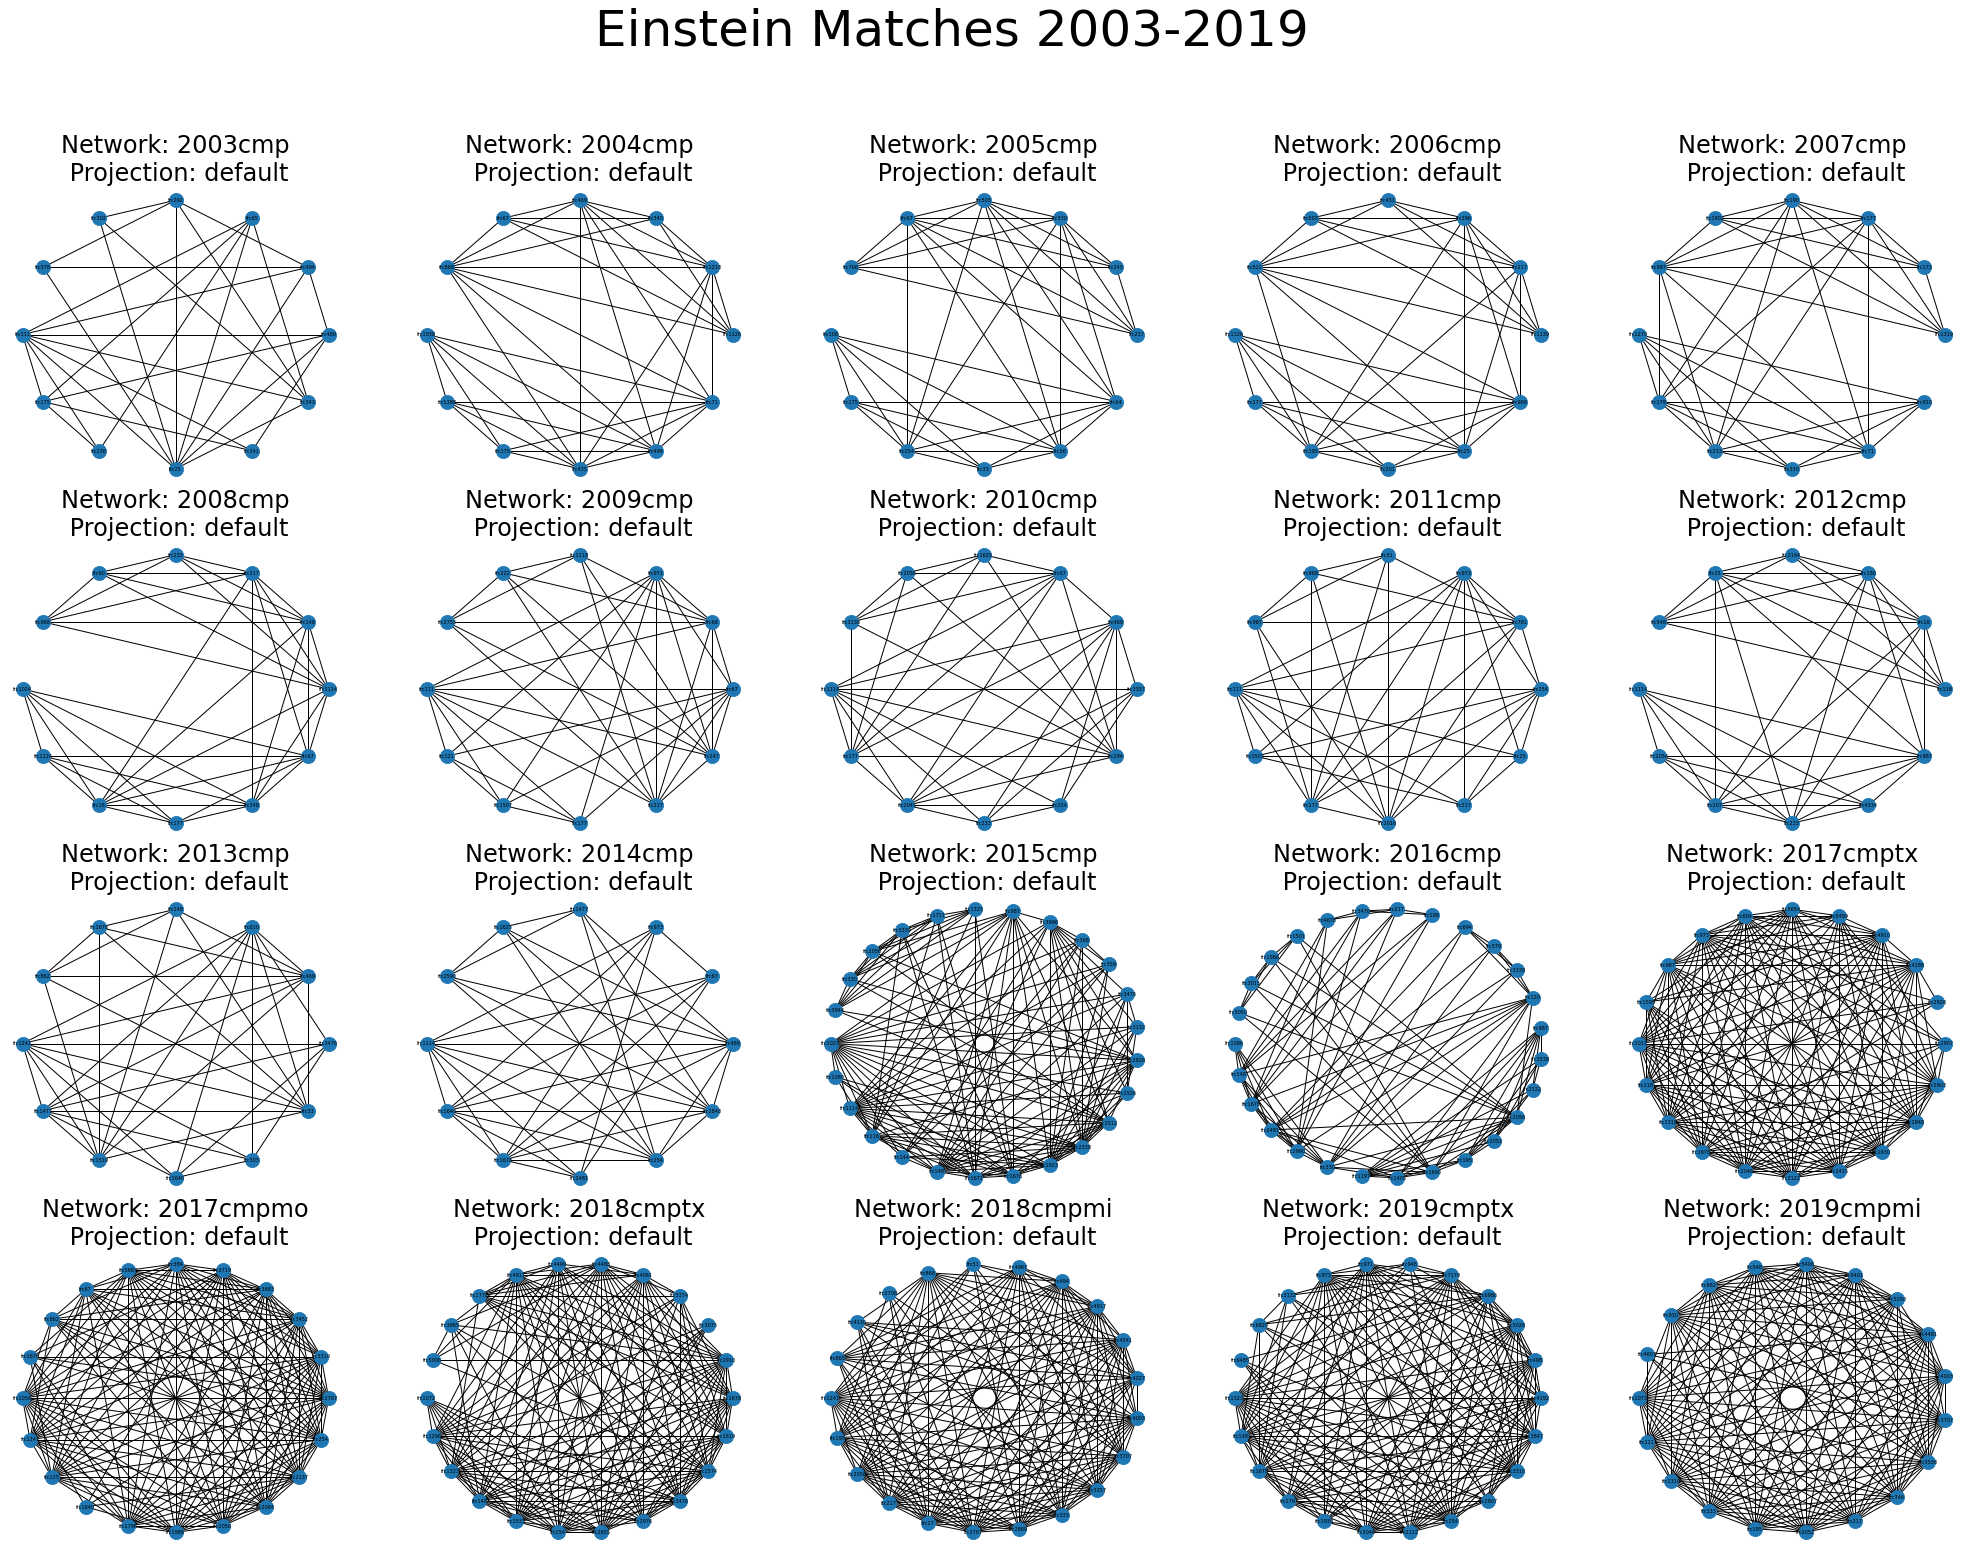
\includegraphics[height=0.9\textheight]{../fig/NetworkPlot_cmp_2003_2019_shell}
\end{frame}

%--------------------------------------------
\begin{frame}{Ending}
	Thanks for listening...\\
	I hope it was was interesting...\\
	Any Questions?
\end{frame}


\begin{frame}[allowframebreaks]{Bibliography}
	Bibliography isn't showing up????
	\begin{itemize}
		\item The Blue Alliance: https://www.thebluealliance.com/
		\item networkx
	\end{itemize}
	\bibliographystyle{unsrt}
	\bibliography{bibliography.bib}
\end{frame}
\end{document}